\section{Google Remote Procedure Call (gRPC)}
Der neue Standard-Technologie für die Backend-Kommunikation in .NET. Primär Server-to-Server Kommunikation im Fokus (Microservices). Hohe Performance von zentraler Bedeutung. Nicht als Frontend-API gedacht. Ist der Ersatz für Windows Communication Foundation.

\begin{description}
  \item[Kommunikationsprotokoll] HTTP/2
  \item[Interface Definition Language] Google Protocol Buffers
\end{description}

\subsection{Architektur}
gRPC ist ein SDK und kann in verschiedene IDEs integriert werden. 

\begin{figure}[h!]
	\centering
	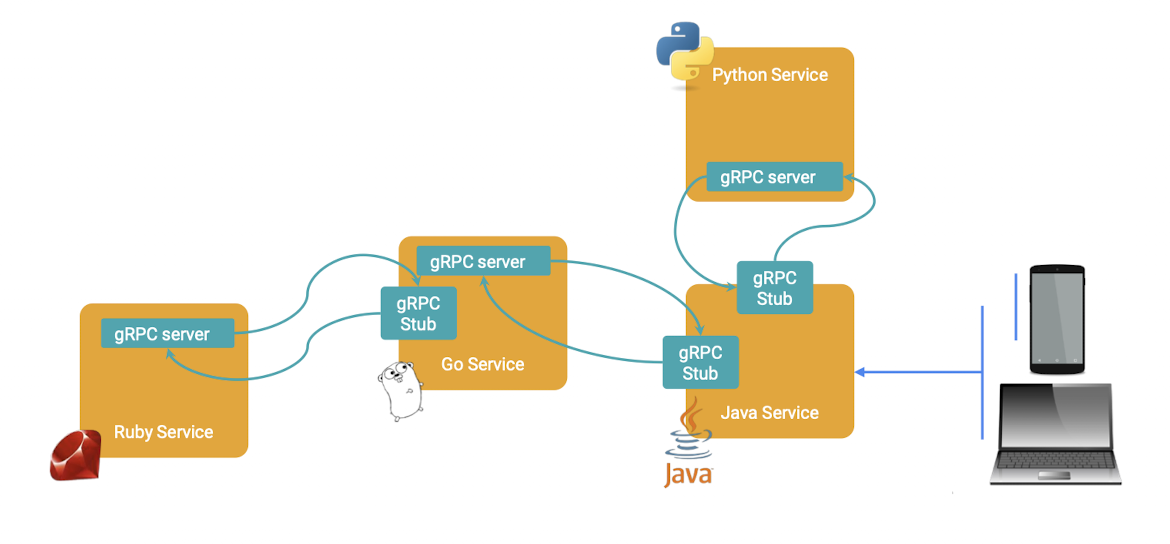
\includegraphics[width=0.75\linewidth]{gRPC}
 	\caption{Architekturbeispeil}
\end{figure}

\begin{figure}[h!]
  	\centering
  	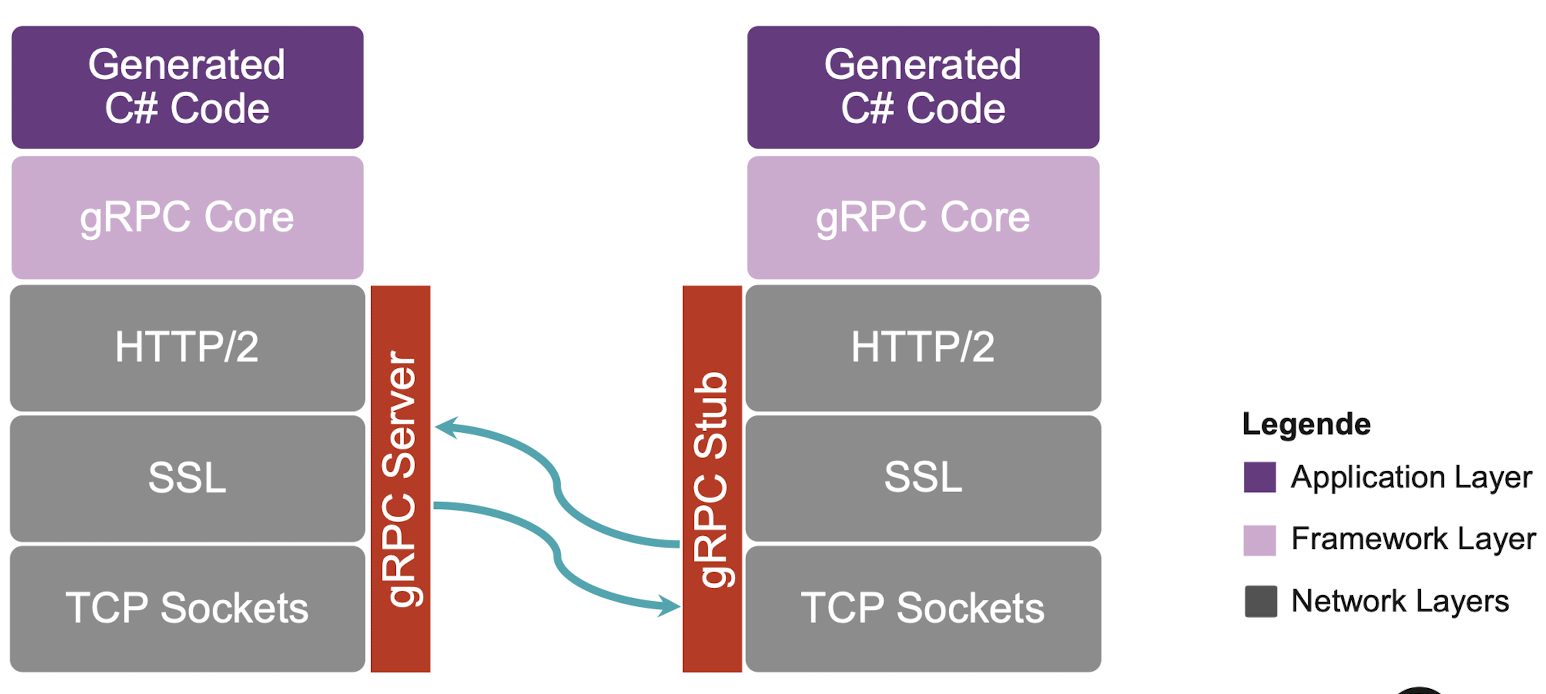
\includegraphics[width=0.5\linewidth]{communicationstack}
  \caption{Kommunikationsstack}
\end{figure}

\textbf{HTTP/2 Features}
\begin{description}
  \item[Multiplexing] Mehrere gRPC Calls pro TCP/IP Session
  \item[Bidirectional Streaming] Asynchronis, nicht-blockierendes Senden und Empfangen von Streams
  \item[HTTPS] HTTP/2 und gRPC basieren voll auf HTTPS $\rightarrow$ Kommunikation ist immer verschlüsselt
\end{description}

\subsection{Protocol Buffers}
\begin{itemize}
  \itemsep -0.5em 
  \item Interface Definition Language (IDL)
  	\SubItem{Ene Subform einer Domain Specific Language (DSL)}
  	\SubItem{Beschreibt ein Service Interface plattform- und sprachneutral.}
  \item Data Model
  	\SubItem{Beschreibt Messages resp. Request- und Response-Objekte}
  \item Wire Format
  	\SubItem{Beschreibt das Binärformat zu Übertragung}
  \item Seriealisierung- und Deserialisierungmechanismen
  \item Service-Versionierung
\end{itemize}

\textbf{Proto Files} \\
Datei-Endung "*.proto". Service-Methoden haben immer einen Parameter und einen Rückgabewert.

\textbf{Messages} \\
Angabe der Feldtypen: Skalarer Typ, Anderer Message Type, Enumeration. Unique Field Name und Unique Field Number.

\subsection{Streams}
Es werden drei Modi untersützt: Server Streaming (Sever - Client), Client Streaming (Client - Server), Bi-directional / Duplex Streaming Call. Es werden zwei verschiedene Modi von Lesen unterstützt: Synchrones und asynchrones lesen.

\subsection{Beispielapplikation}

\pagebreak
  









